\documentclass[a4paper,12pt]{article}
\usepackage[utf8]{inputenc} % Kodowanie UTF-8
\usepackage[T1]{fontenc}    % Lepsza obsługa polskich znaków
\usepackage[polish]{babel}  % Polskie znaki i ustawienia językowe
\usepackage{graphicx}
\usepackage{amsmath}
\usepackage{caption}
\usepackage{subcaption}
\usepackage{geometry}
\geometry{margin=1in}


\title{Sprawozdanie: Analiza Błędów Sumowania w $n$-Kącie}
\author{Tymoteusz Herkowiak, Marcin Panasko}
\date{17.03.2025}

\begin{document}

\maketitle

\begin{abstract}
W tej pracy zbadaliśmy, jak błędy w obliczeniach komputerowych wpływają na sumowanie wektorów w wielokącie foremnym. Suma powinna być bliska zera, ale przez ograniczenia komputera pojawiają się małe błędy. Sprawdziliśmy trzy hipotezy (H1-H3), żeby zobaczyć, jak różne sposoby sumowania radzą sobie z tym problemem.
\end{abstract}

\section{Wyniki i Analiza}

\subsection{Konstrukcja wierzchołków (H1)}

Na początek obliczyliśmy wierzchołki wielokąta foremnego, zaczynając od punktu \( \mathbf{v}_0 = (1,0) \). W idealnym świecie, po dodaniu wszystkich wektorów \( \mathbf{w}_i \), powinniśmy wrócić dokładnie do tego samego miejsca, czyli \( \mathbf{v}_n = \mathbf{v}_0 \).  Przez ograniczenia w dokładności (używamy typu \texttt{double}) i małe błędy w obliczeniach funkcji takich jak \( \cos() \) czy \( \sin() \), końcowy punkt trochę różni się od startowego. 

Te różnice są bardzo małe – mieszczą się w granicach od \( 10^{-15} \) do \( 10^{-14} \), co jest normalne dla takich obliczeń.

\subsection{Błędy sumowania (H2, H3)}

Sprawdziliśmy dwa sposoby sumowania wektorów:  
- H2 – dodajemy w kolejności, w jakiej są podane,  
- H3 – najpierw sortujemy wektory, a potem je sumujemy.  

Wyniki pokazaliśmy na wykresach poniżej (Rysunek~\ref{fig:errors}).

\begin{figure}[h]
    \centering
    \begin{subfigure}[b]{0.45\textwidth}
        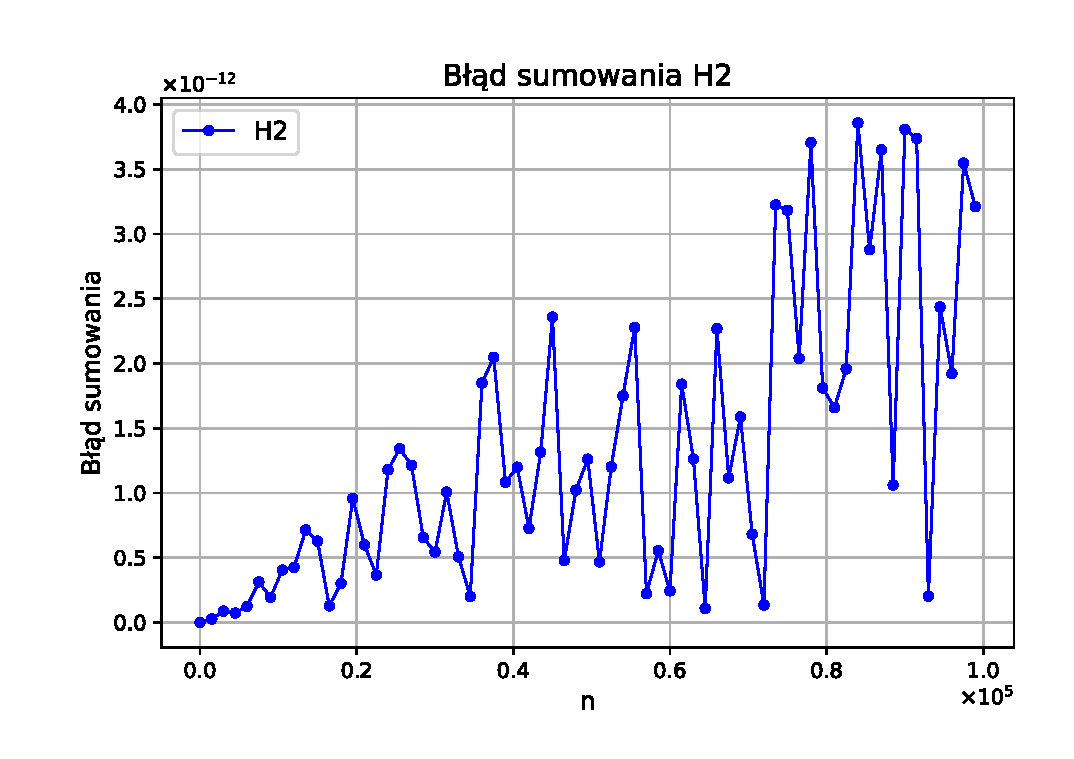
\includegraphics[width=\textwidth]{blad_sumowania_h2.pdf}
        \caption{H2}
    \end{subfigure}
    \hfill
    \begin{subfigure}[b]{0.45\textwidth}
        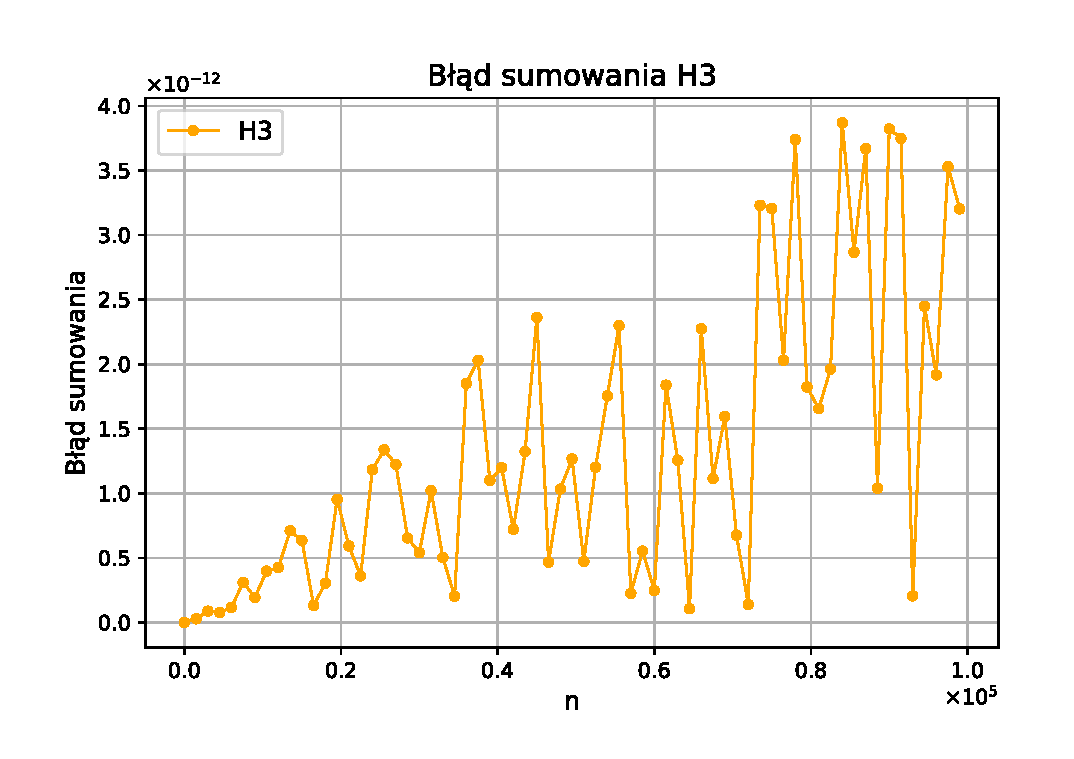
\includegraphics[width=\textwidth]{blad_sumowania_h3.pdf}
        \caption{H3}
    \end{subfigure}
    \caption{Błędy sumowania dla różnych \( n \)}
    \label{fig:errors}
\end{figure}

\textbf{-Wykres H2 (lewy):}
 Błąd w metodzie H2 zmienia się od 0 do \( 4 \times 10^{-12} \). Na początku, przy małych wartościach \( n \) (do 20000), błąd jest prawie zerowy. Potem rośnie, szczególnie w okolicach \( n = 0.8 \times 10^5 \), gdzie osiąga najwyższe wartości. Później się uspokaja i oscyluje między \( 1 \times 10^{-12} \) a \( 2 \times 10^{-12} \). To pokazuje, że im więcej liczb sumujemy, tym bardziej błąd może się zmieniać. Dla niektórych wartości n błąd pozostaje niski, co pokazuje, że zależność ta nie jest liniowa.

\textbf{-Wykres H3 (prawy):} Błąd w metodzie H3 też mieści się w granicach od 0 do \( 4 \times 10^{-12} \). Wygląda bliźniaczo do H2.

\textbf{Podsumowanie:} Obie metody mają błędy rzędu \( 10^{-12} \), obie metody wydają się dawać bliźniacze efekty, nie można stwierdzić większej dokładności którejś z nich na podstawie tych wykresów.


\subsection{Stosunek błędów (H3/H2)}

Porównaliśmy, jak bardzo różnią się błędy między metodami H3 i H2, dzieląc błąd H3 przez błąd H2. Wyniki pokazano na Rysunku~\ref{fig:ratio}.

\begin{figure}[h]
    \centering
    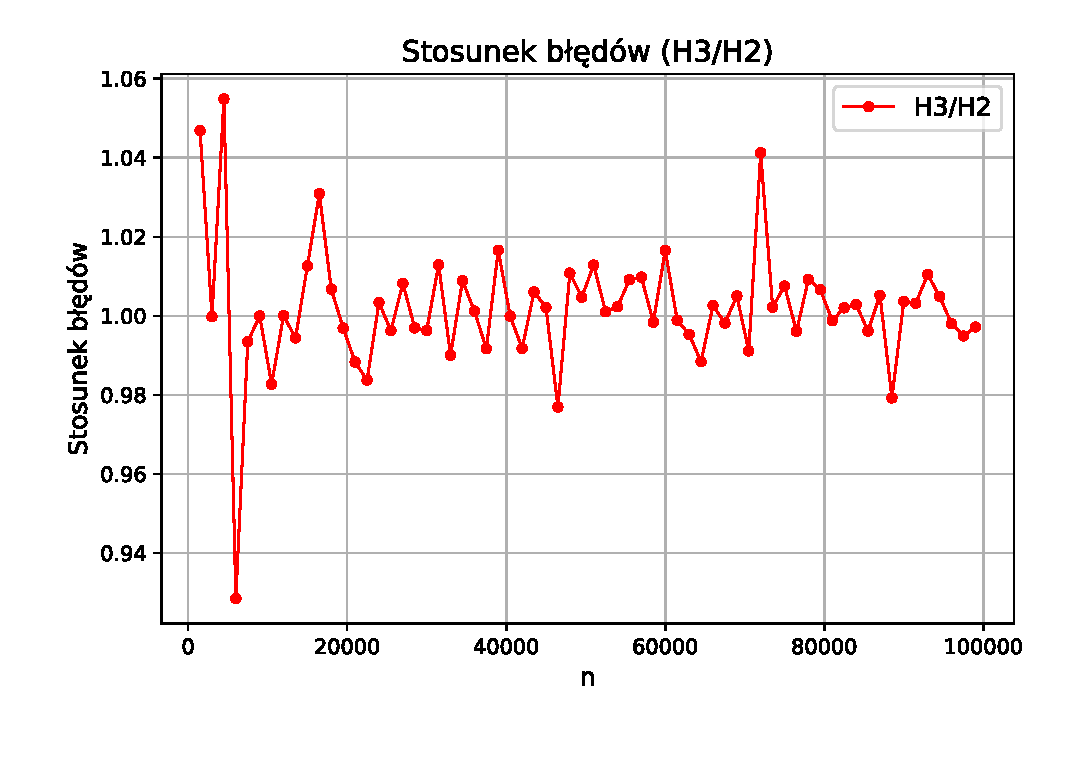
\includegraphics[width=0.6\textwidth]{stosunek_bledow_h3h2.pdf}
    \caption{Stosunek błędów \( \frac{H3}{H2} \) .}
    \label{fig:ratio}
\end{figure}

\begin{itemize}
    \item Stosunek \( \frac{H3}{H2} \) zmienia się od około 0.92 do 1.06.
    \item Dla większości wartości \( n \) jest bardzo blisko 1, co oznacza, że obie metody dają podobne wyniki.
    \item Są jednak miejsca, gdzie H3 daje większy błąd – na przykład przy \( n = 0.72 \times 10^5 \) i w okolicach 0, stosunek dochodzi do 1.06, czyli H3 ma błąd o 6\% większy niż H2.
    \item Czasem H3 jest lepsze, bo stosunek spada do 0.94, ale te różnice są naprawdę małe i nie wskazują na wyraźną przewagę jednej metody.


\end{itemize}

\subsection{Różnice błędów (H2 – H3)}

Sprawdziliśmy, o ile błąd H2 różni się od błędu H3, odejmując je od siebie. Wyniki pokazano na Rysunku~\ref{fig:difference}.

\begin{figure}[h]
    \centering
    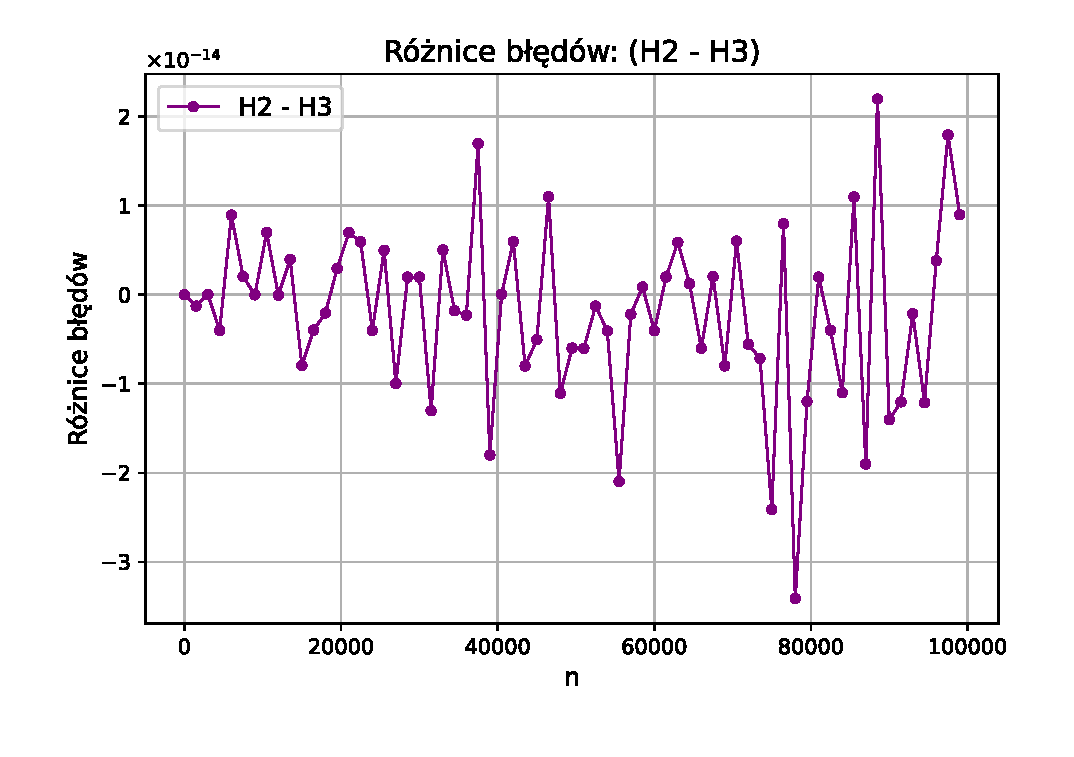
\includegraphics[width=0.6\textwidth]{roznice_bledow_h2h3.pdf}
    \caption{Różnice błędów \( H2 - H3 \)}
    \label{fig:difference}
\end{figure}

\begin{itemize}
    \item Różnice \( H2 - H3 \) mieszczą się w granicach od \( -4 \times 10^{-14} \) do \( 3 \times 10^{-14} \).
    \item Kiedy różnica jest ujemna (np. przy \( n = 0.88 \times 10^5 \)), oznacza to, że H3 daje większy błąd niż H2.
    \item Kiedy różnica jest dodatnia (np. przy ok. \( n = 0.38 \times 10^5 \)), to H2 ma większy błąd.
    \item Te różnice są bardzo małe, więc obie metody działają podobnie.
\end{itemize}

\section{Podsumowanie Wyników}

Z naszych obliczeń wynika, że błędy w obu metodach (H2 i H3) mieszczą się w granicach od 0 do \( 10^{-12} \), czyli są bardzo małe i bliskie temu, co komputer może dokładnie policzyć (typ \texttt{double}). Metoda H3 czasem daje trochę większy błąd niż H2, a czasem mniejszy, ale różnice nie są duże. Gdyby suma nie była tak bliska zeru, różnice między metodami mogłyby być łatwiejsze do zauważenia.

\section{Wnioski}

W naszym przypadku, gdzie suma wektorów jest prawie zerowa, obie metody (H2 i H3) działają bardzo podobnie – żadna nie jest wyraźnie lepsza. Błędy są na poziomie, który wynika z ograniczeń komputera, więc nie da się ich bardziej zmniejszyć bez zmiany sposobu obliczeń. 

\section*{Uwagi}
Zakres pracy członków zespołu:
\begin{itemize}
    \item Kod w C zrobiliśmy prawie cały wspólnie na zajęciach, wymieniając się uwagami i wprowadzając poprawki. Później jedynie dostosowaliśmy wielkość n oraz sposób zapisu danych do pliku na potrzeby skryptu w Pythonie tworzącego wykresy.
    \item Zaczeliśmy prace nad skryptem w Pythonie wspólnie, po czym Tymoteusz zajął się dostosowaniem outputu kodu w C do potrzeb Pythona zgodnie z naszym konceptem, a Marcin kontynuował pracę nad kodem Pythona tworzącym wykresy. Na koniec wspólnie dostosowywaliśmy wielkość i przeskoki między kolejnymi n na potrzeby czytelności wykresów.
    \item Tworząc sprawozdanie podzieliliśmy się po połowie, Tymoteusz zrobił Wstęp i 1.1, 1.2, Marcin 1.3, 1.4, Podsumowanie.
\end{itemize}

\end{document}